\section{Experiments}
\label{sec:experiments}

\begin{figure*}[t]
\centering
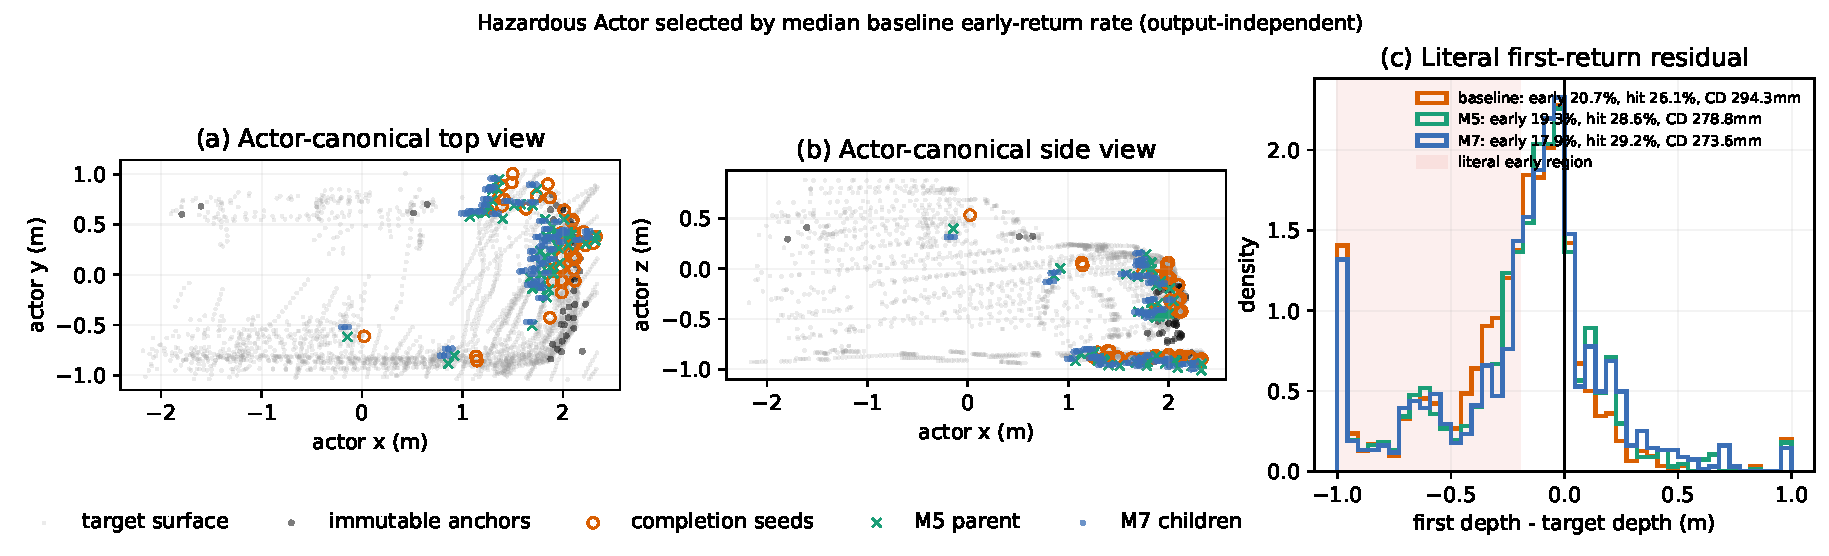
\includegraphics[width=\textwidth]{figures/v71_m7_supervision_native_geometry.pdf}
\caption{Canonical set expansion on a hazardous development Actor. The 47 completion seeds produce 188 children
while observed anchors stay fixed. Original/relocation/set-expansion early rates are 20.7/19.3/17.9\%,
hit rates are 26.1/28.6/29.2\%, and Chamfer distances are 294.3/278.8/273.6\,mm.
Gray points are disjoint target observations. This example shows the set-expansion stage before frame fine-tuning.}
\label{fig:v71-m7-geometry}
\end{figure*}

\subsection{Experimental Setup}

\paragraph{Data.}
We use nuScenes~\cite{caesar2020nuscenes} for learning and Argoverse~2 Sensor validation
\cite{wilson2021argoverse2} for the frozen external evaluation.
The geometry and evidence stages use 593 training Actors and a 66-Actor development fold
(41 hazardous, 25 clear; 99,208 rays). The fold was exposed during predecessor development,
so source results characterize the learned mechanism.
AV2 selection excludes the 60 logs used by the earlier compiler studies from 150 validation logs.
Positions $0,4,\ldots,76$ in the sorted 90-log complement give 20 logs, 352 Actors, and 1,016,652 rays.
Models, transforms, and evaluation parameters are frozen before this evaluation.

\paragraph{Metrics and implementation.}
Early and hit rates use all target rays as their denominator; misses remain in that denominator.
Chamfer is the Actor-mean symmetric nearest-neighbor distance.
We report all, hazardous, and clear strata. Surface comparisons use literal beam-tube returns;
evidence comparisons use interpolated categorical returns on identical geometry.
All Actor states are retained.
The four-child decoder has hidden width 128 and 16-dimensional slots; frame-aware fine-tuning runs
six epochs with AdamW, learning rate $10^{-4}$, and four Actors per batch.
Evidence heads use hidden width 64. The local archive gives their staged training schedule and run identities.

\subsection{Canonical Surface Reconstruction}

Table~\ref{tab:eas-geometry} compares the original completion surface with target-set expansion and
its frame-balanced extension. Set expansion reduces hazardous early returns from 27.80\% to 24.96\%,
improves Chamfer by 2.90\,mm, and increases hit recall by 2.17 points.
Frame coverage further improves Chamfer to 231.46\,mm and hit recall to 50.43\%.
It also reduces frame-mean target distance by 7.01\,mm for moving Actors and 3.55\,mm for quasi-static Actors
relative to set expansion. Its hazardous early rate is 26.37\%, a 5.12\% relative reduction from the original surface.

\begin{table}[t]
\centering\footnotesize
\setlength{\tabcolsep}{3pt}
\caption{Canonical geometry on 66 development Actors. Early and hit are ray percentages; CD is Actor-mean Chamfer in mm.
All rows use literal point-surface returns and retain 100\% of Actor states.}
\label{tab:eas-geometry}
\begin{tabular}{lrrrrr}
\toprule
& \multicolumn{3}{c}{Early $\downarrow$} & CD $\downarrow$ & Hit $\uparrow$\\
Method & All & Hazard & Clear & (mm) & (\%)\\
\midrule
Original & 26.74 & 27.80 & \textbf{21.56} & 237.67 & 47.67 \\
Set expansion & \textbf{24.41} & \textbf{24.96} & 21.74 & 234.77 & 49.84 \\
+ frame coverage & 25.70 & 26.37 & 22.39 & \textbf{231.46} & \textbf{50.43} \\
\bottomrule
\end{tabular}
\end{table}


Frame coverage therefore improves the completeness side of the trade-off while retaining the hazardous
early-return improvement over the baseline. Clear early returns rise from 21.56\% to 22.39\%;
the stratified table makes this trade-off explicit.
Figure~\ref{fig:v71-m7-geometry} visualizes set expansion on an Actor chosen by its baseline early-return
median before inspecting learned output. The additional children cover the held-out surface more closely.


\subsection{Evidence and Return Composition}

Producer replay aligns 297,535 anchors across 1,004 corpus Actors with build and target ray evidence.
Build and target occupied masses correlate at $r=0.514$, while 58.72\% of anchors receive both free
and occupied target votes. This supplies a predictive but contradictory observation history for the evidence heads.

Table~\ref{tab:eas-return} isolates the effect of learned evidence on fixed frame-supervised geometry.
The categorical measure lowers early rate from 18.19\% to 17.67\% and raises hit recall from 62.28\% to 64.46\%.
Hazardous early rate decreases by 0.62 points and hazardous hit recall increases by 2.32 points.
All three strata improve both metrics. The clear early decrease is small (0.03 points);
the larger gains occur in hit recall.

\begin{table}[t]
\centering\footnotesize
\setlength{\tabcolsep}{5pt}
\caption{Categorical return comparison on identical geometry within each dataset. Unit: unit Gaussian energy.
EAS: learned evidential weights. All values are percentages; source and AV2 are distinct cohorts.}
\label{tab:eas-return}
\begin{tabular}{lrrrr}
\toprule
& \multicolumn{2}{c}{Early $\downarrow$} & \multicolumn{2}{c}{Hit $\uparrow$}\\
Stratum & Unit & EAS & Unit & EAS\\
\midrule
\multicolumn{5}{l}{\emph{nuScenes development: 66 Actors / 99,208 rays}}\\
All & 18.19 & \textbf{17.67} & 62.28 & \textbf{64.46} \\
Hazardous & 17.42 & \textbf{16.80} & 62.07 & \textbf{64.39} \\
Clear & 21.95 & \textbf{21.92} & 63.34 & \textbf{64.80} \\
\midrule
\multicolumn{5}{l}{\emph{AV2 frozen: 352 Actors / 1,016,652 rays}}\\
All & 16.91 & 17.14 & 38.35 & 44.24 \\
Hazardous & 16.56 & 17.10 & 27.98 & 34.28 \\
Clear & 17.21 & 17.17 & 47.14 & 52.68 \\
\bottomrule
\end{tabular}
\end{table}


\paragraph{Why the composition matters.}
Using the same learned anchor and child evidence as additive transmittance gives 21.51\% early returns
and 66.92\% hit recall. Categorical composition shifts this operating point to 17.67\%/64.46\%.
The ordered optical model is therefore useful for learning evidence, but its accumulated front-tail mass
produces earlier returns on this primitive set.
An exact responsibility audit finds that the categorical model reduces mean pre-boundary mass by 0.331 points:
anchors contribute $-0.346$ points and children $+0.016$ points.
The observed-anchor evidence accounts for most of the net reduction.

\subsection{Attenuation and First-Return Behavior}

Figure~\ref{fig:m49-sign-boundary} evaluates Eq.~\ref{eq:finite-attenuation-boundary} on 99,208 frozen rays.
Uniform child attenuation has the adverse sign on 58.85\% of rays and the favorable sign on 30.96\%.
For a learned component-wise visibility ablation, exact pre-boundary mass increases on 59.32\% of rays
and decreases on 27.27\%. The first-order prediction agrees with the finite-change sign on 95.73\%.
These observations illustrate the distinction between reducing a component's weight and reducing the
normalized mixture's probability before a boundary.

\begin{figure}[t]
\centering
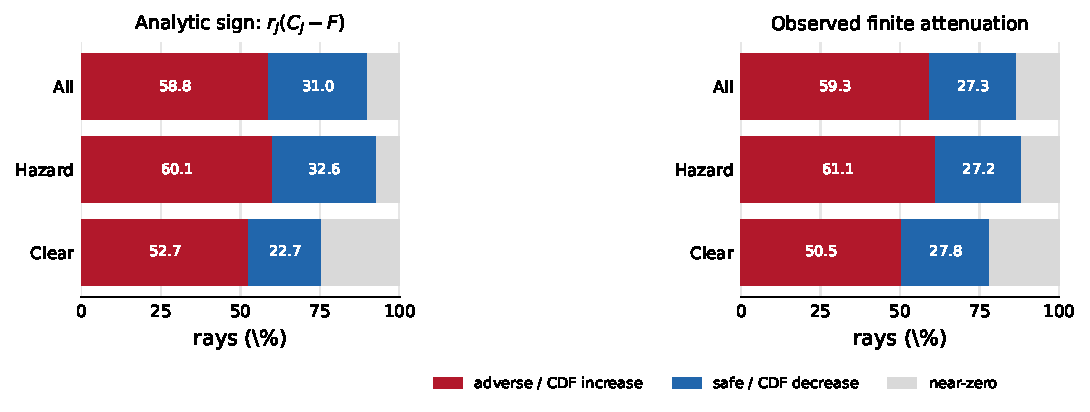
\includegraphics[width=\linewidth]{figures/v71_m49_attenuation_sign_boundary.pdf}
\caption{Attenuation response on frozen development rays. Left: sign predicted for uniform child attenuation.
Right: exact change under the learned visibility ablation. Red indicates increased pre-boundary probability;
blue indicates a decrease.}
\label{fig:m49-sign-boundary}
\end{figure}

The smooth ray loss has a related operator boundary: expected-depth error does not determine the literal
minimum over supported centers. In a frame-balanced ray-loss ablation, 38.03\% of newly early rays improve
their smooth depth error even when both operators use exactly the same support.
The local archive gives a constructive counterexample and the full same-support/deployment comparison.

\subsection{Dynamic Scene Composition}

We match 12 scene-0230 Actors to a read-only StreetGS checkpoint.
Across 36 Actor--frames, 5,791 physical Gaussians follow rigid poses independently of 106,807 appearance-owned
and 1,140,862 Background Gaussians.
The unit-weight composition audit yields maximum energy and pairwise-distance residuals of
$3.40\times10^{-14}$ and $1.24\times10^{-14}$\,m under translations up to 126.28\,m.
This verifies the coordinate composition in Eq.~\ref{eq:authority-query}.
Separate visual-parameter optimization leaves physical centers and scales fixed, validating the gradient ownership
used by the scene interface. The archive reports the associated appearance-capacity experiments.

\subsection{Cross-Sensor Evaluation}

On the frozen AV2 cohort, the categorical model increases overall hit recall from 38.35\% to 44.24\%
and hazardous hit recall from 27.98\% to 34.28\% (Table~\ref{tab:eas-return}).
Early rates rise by 0.23 points overall and 0.54 points for hazardous Actors.
The all-early and worst-stratum nonincrease criteria consequently fail, while hit retention passes.
The complete result shows a source-to-target trade-off: the return measure recovers more measured endpoints,
but its source-domain early-return improvement does not transfer.
No AV2 fine-tuning, calibration, or threshold adjustment is applied.
